% To make this maximally compatible with older PDF readers, it uses
% PDF 1.4 and TeXGyre fonts
\pdfminorversion=4
\documentclass{ltxdockit}
\usepackage[british]{babel}
\usepackage[strict=true,autostyle=true]{csquotes}
\usepackage{ifthen}
\usepackage{fontspec}
\usepackage{tikz}
\usepackage{graphicx}
\usepackage{booktabs}
\usepackage{fixfoot}
\usepackage{color}
\usepackage{listings}
\usepackage{metalogo}
\usepackage[retainmissing]{MnSymbol}
\setmainfont[Ligatures=TeX]{TeXGyrePagella}
\setsansfont[Ligatures=TeX]{TexGyreHeros}
\setmonofont[Ligatures=NoCommon]{TeXGyreCursor}

\renewcommand{\labelitemii}{$\circ$}

\MakeAutoQuote{«}{»}

\gdef\biberversion{0.9.8}    % BIBER VERSION
\gdef\biblatexversion{1.7}   % BIBLATEX VERSION

% Set up tikz things

\usetikzlibrary{shapes.geometric}
\usetikzlibrary{arrows}
\usetikzlibrary{fit}
\usetikzlibrary{calc}
\tikzstyle{file} = [rectangle, black, very thick, draw=blue, fill=blue!20,
                    minimum width=6em, minimum height=3em, align=center]
\tikzstyle{funit} = [rectangle, rounded corners=1ex, black, very thick,
                     shape border rotate=-90, draw=green, fill=green!20,
                     minimum size=3em, align=center]

% colours for the .dot examples
\xdefinecolor{centry}{HTML}{A0D0FF}
\xdefinecolor{ncentry}{HTML}{DEEFFF}
\xdefinecolor{doentry}{HTML}{FDFFD9}
\xdefinecolor{section}{HTML}{FCE3FA}
\xdefinecolor{set}{HTML}{E3DADC}
\xdefinecolor{related}{HTML}{AD1741}
\xdefinecolor{clone}{HTML}{AD1741}
\xdefinecolor{crossref}{HTML}{7D7879}
\xdefinecolor{xref}{HTML}{7D7879}
\xdefinecolor{xdata}{HTML}{2CA314}

\DeclareFixedFootnote{\tpb}{Binary maintained by third party. See README in
  binary download directory for this platform for support/contact
  details. Usually, the binary maintainer is also the binary build
  provider for \TeX Live.}

\titlepage{%
  title={biber},
  subtitle={A backend bibliography processor for biblatex},
  url={http://biblatex-biber.sourceforge.net},
  author={François Charette, Philip Kime},
  email={firmicus@ankabut.net, Philip@kime.org.uk},
  revision={biber \biberversion\ (biblatex \biblatexversion)},
  date={\today}}

\hypersetup{%
  pdftitle={biber},
  pdfsubject={A backend bibliography processor for biblatex},
  pdfauthor={Philip Kime},
  pdfkeywords={biblatex, bibliography}}


% Control list spacing
\usepackage{enumitem}
\setdescription{noitemsep}
\setenumerate{noitemsep}
\setitemize{noitemsep}

\def\biberex#1{\hbox{\hspace{-4em}\texttt{\small \detokenize{#1}}}}

\begin{document}
\definecolor{grey}{rgb}{0.7,0.7,0.7}
\printtitlepage
\tableofcontents

\section{Important Changes}\label{special}

Please see the \verb+Changes+ file which accompanies Biber for the
details on changes in each version. This section is just for important
things like incompatible changes which users should be aware of.

\minisec{0.9.7}
\textcolor{red}{The user config file has a completely new format}.The
  reason for this is that the older \verb+Config::General+ format
  could not be extended to deal with more sophisticated features like
  per-datasource restrictions. An XML format is much better and in
  fact easier to understand. The old format of the \verb+map+ option
  (now called \verb+sourcemap+) was rather confusing because
  of limitations in the old config file format. Please see section
  \ref{map} and convert your config files to the new format.

\minisec{0.9.6}
\textcolor{red}{Matching of citation keys and datasource entry keys is now
  \emph{case-sensitive}}. This is to enforce consistency across the entire
Bib\LaTeX\ and Biber processing chain. All of the usual referencing
mechanisms in \LaTeX\ are case-sensitive and so is the matching in
Bib\LaTeX\ of citations to entries in the \texttt{.bbl} file generated by
Biber. It is inconsistent and messy to enforce case-insensitivity in only
Biber's matching of citations keys to datasource entry keys. If Biber
detects what looks like a case mismatch between citation keys, it will warn
you.

\noindent \textcolor{red}{Summary of warnings/errors is now a new format}.
When Biber finishes writing the \verb+.bbl+, it gives a summary
count of errors/warnings. It used to do this in the same format as
Bib\TeX, for compatibility. Now it uses a more consistent and easier
to parse format which matches all other Biber messages. Please note
if you need to support Biber in an external tool. I have updated the
notes on AUC\TeX\ support below to reflect this.

\section{Introduction}\label{int}

\subsection{About}

Biber is conceptually a Bib\TeX\ replacement for
Bib\LaTeX. It is written in Perl with the aim of providing a
customised and sophisticated data preparation backend for Bib\LaTeX.
You do \emph{not} need to install Perl use Biber---binaries
are provided for many operating systems via the main \TeX\
distributions (\TeX Live, Mac\TeX, MiK\TeX) and also via download from SourceForge.
Functionally, Biber offers a superset of Bib\TeX's capabilities but is
tightly coupled with Bib\LaTeX\ and cannot be used as a stand-alone tool
with standard \verb+.bst+ styles. Biber's role is to support
Bib\LaTeX\ by performing the following tasks:

\begin{itemize}
\item Parsing data from data sources
\item Processing cross-references, entry sets, related entries
\item Generating data for name, name list and name/year disambiguation
\item Structural validation according to Bib\LaTeX\ data model
\item Sorting reference lists
\item Outputting data to a \verb+.bbl+ for Bib\LaTeX\ to consume
\end{itemize}

\subsection{Requirements}\label{ref:req}

Biber is distributed primarily as a stand-alone binary and is
included in \TeX Live, Mac\TeX\ and MiK\TeX. If you are using any of these
distributions, you do not need any additional software installed to use
Biber. You do \emph{not} need a Perl installation at all to use
the binary distribution of Biber\footnote{If you prefer, you can run
Biber as a normal Perl program and doing this \emph{does} require
you to have a Perl interpreter installed. See section \ref{binaries}.}.

Biber's git repository is on
github\footnote{\url{https://github.com/plk/biber}}. Biber's documentation,
binary downloads and supporting files are on
SourceForge\footnote{\url{http://sourceforge.net/projects/biblatex-biber/}}
and this is the primary location for development releases, forums and
bugfixes etc. Biber is included into \TeX Live, the binaries coming from
SourceForge.

\subsection{Compatibility Matrix}

Biber versions are closed coupled with Bib\LaTeX\ versions. You
need to have the right combination of the two. Biber will warn you
during processing if it encounters information which comes from the wrong
Bib\LaTeX\ version. Table \ref{tab:compat} shows a compatibility
matrix for the recent versions.

\begin{table}
\begin{center}
\small
\begin{tabular}{lllll}
\toprule
Biber version & Bib\LaTeX\ version\\
\midrule
0.9.7 & 1.7x\\
0.9.6 & 1.7x\\
0.9.5 & 1.6x\\
0.9.4 & 1.5x\\
0.9.3 & 1.5x\\
0.9.2 & 1.4x\\
0.9.1 & 1.4x\\
0.9 & 1.4x\\
\bottomrule
\end{tabular}
\end{center}
\caption{Biber/Bib\LaTeX\ compatibility matrix}
\label{tab:compat}
\end{table}

\subsection{License}

Biber is released under the free software Artistic License 2.0\footnote{\url{http://www.opensource.org/licenses/artistic-license-2.0.php}}

\subsection{History}

Bib\TeX\ has been the default (only \ldots) integrated choice for
bibliography processing in \TeX\ for a long time. It has well known
limitations which stem from its data format, data model and lack of Unicode
support\footnote{In fact, there is now a Unicode version}. The
\verb+.bst+ language for writing bibliography styles is painful to learn
and use. It is not a general programming language and this makes it really
very hard to do sophisticated automated processing of bibliographies.

Bib\LaTeX\ was a major advance for \LaTeX\ users as it moved much
of the bibliography processing into \LaTeX\ macros. However,
Bib\LaTeX\ still used Bib\TeX\ as a sorting engine for the
bibliography and also to generate various labels for
entries. Bib\TeX's capabilities even for this reduced set of
tasks was still quite restricted due to the lack of Unicode support and
the more and more complex programming issues involved in label
preparation and file encoding.

Biber was designed specifically for Bib\LaTeX\ in order to
provide a powerful backend engine which could deal with any required
tasks to do with \verb+.bbl+ preparation. Its main features are:

\begin{itemize}
\item Deals with the full range of UTF-8
\item Sorts in a completely customisable manner using, when available,
  CLDR collation tailoring
\item Allows for per-entrytype options
\item Automatically encodes the \verb+.bbl+ into any supported encoding
  format\footnote{«Supported» here means encodings supported by the
    Perl \texttt{Encode} module}
\item Processes all bibliography sections in one pass of the tool
\item Handles UTF-8 citekeys and filenames (given a suitable fully
  UTF-8 compliant \TeX\ engine)
\item Creates entry sets dynamically and allows easily defined static entry sets,
  all processed in one pass
\item «Syntactic» inheritance via new \verb+XDATA+ entrytype and
  field. This can be thought of as a field-based generalisation of the
  Bib\TeX\ \verb+@STRING+ functionality (which is also supported).
\item «Semantic» inheritance via a generalisation of the Bib\TeX\
  crossreference mechanism. This is highly customisable by the
  user---it is possible to choose which fields to inherit for which
  entrytypes and to inherit fields under different names etc.
\item Handles complex auto-expansion and contraction of names and
  namelists (See section 4.11.4 of the Bib\LaTeX\ manual for an excellent
  explanation with examples, this is quite an impressive feature \ldots)
\item Extensible modular data sources architecture for ease of adding
  more data source types
\item Support for remote data sources
\item User-definable mapping and suppression of fields and entrytypes in
  data sources. You can use this to, for example, ignore all
  \verb+ABSTRACT+ fields completely. See section \ref{map}
\item Support for related entries, to enable generic treatment of things
  like «translated as», «reprinted as», «reprint of»
  etc. (Bib\LaTeX\ support coming in Bib\LaTeX\ 2.x)
\item Customisable labels (Bib\LaTeX\ support coming in
  Bib\LaTeX\ 2.x)
\item Multiple bibliography lists in the same section with different
  sorting and filtering (Bib\LaTeX\ support coming in Bib\LaTeX\ 2.x)
\item No more restriction to a static data model of specific fields and
  entrytypes. (Bib\LaTeX\ support coming in Bib\LaTeX\ 2.x)
\item Structural validation of the data against the data model with a
  customisable validation model (Bib\LaTeX\ support coming in
  Bib\LaTeX\ 2.x)
\end{itemize}

\noindent Figure \ref{fig:overview} shows the main functional units of
processing in Biber. The most difficult tasks which Biber
performs are the processing of Bib\LaTeX's \verb+uniquename+ and
\verb+uniquelist+ options\footnote{A rather tricky unbounded loop but with
  a guaranteed eventual stable exit state.}, the sorting of
lists\footnote{This is a complex, arbitrary multi-field Schwartzian
  Transform which has to deal with potentially different case and order
  settings for every field.} and the initial data parse and remap into an
internal data model. Biber is getting on for around 20,000 lines of
mostly OO Perl and relies on certain splendid Perl modules
such as \verb+Unicode::Collate+, \verb+Text::BibTeX+ and
\verb+XML::LibXML+.

\begin{figure}[!htpb]
  \centering\small
  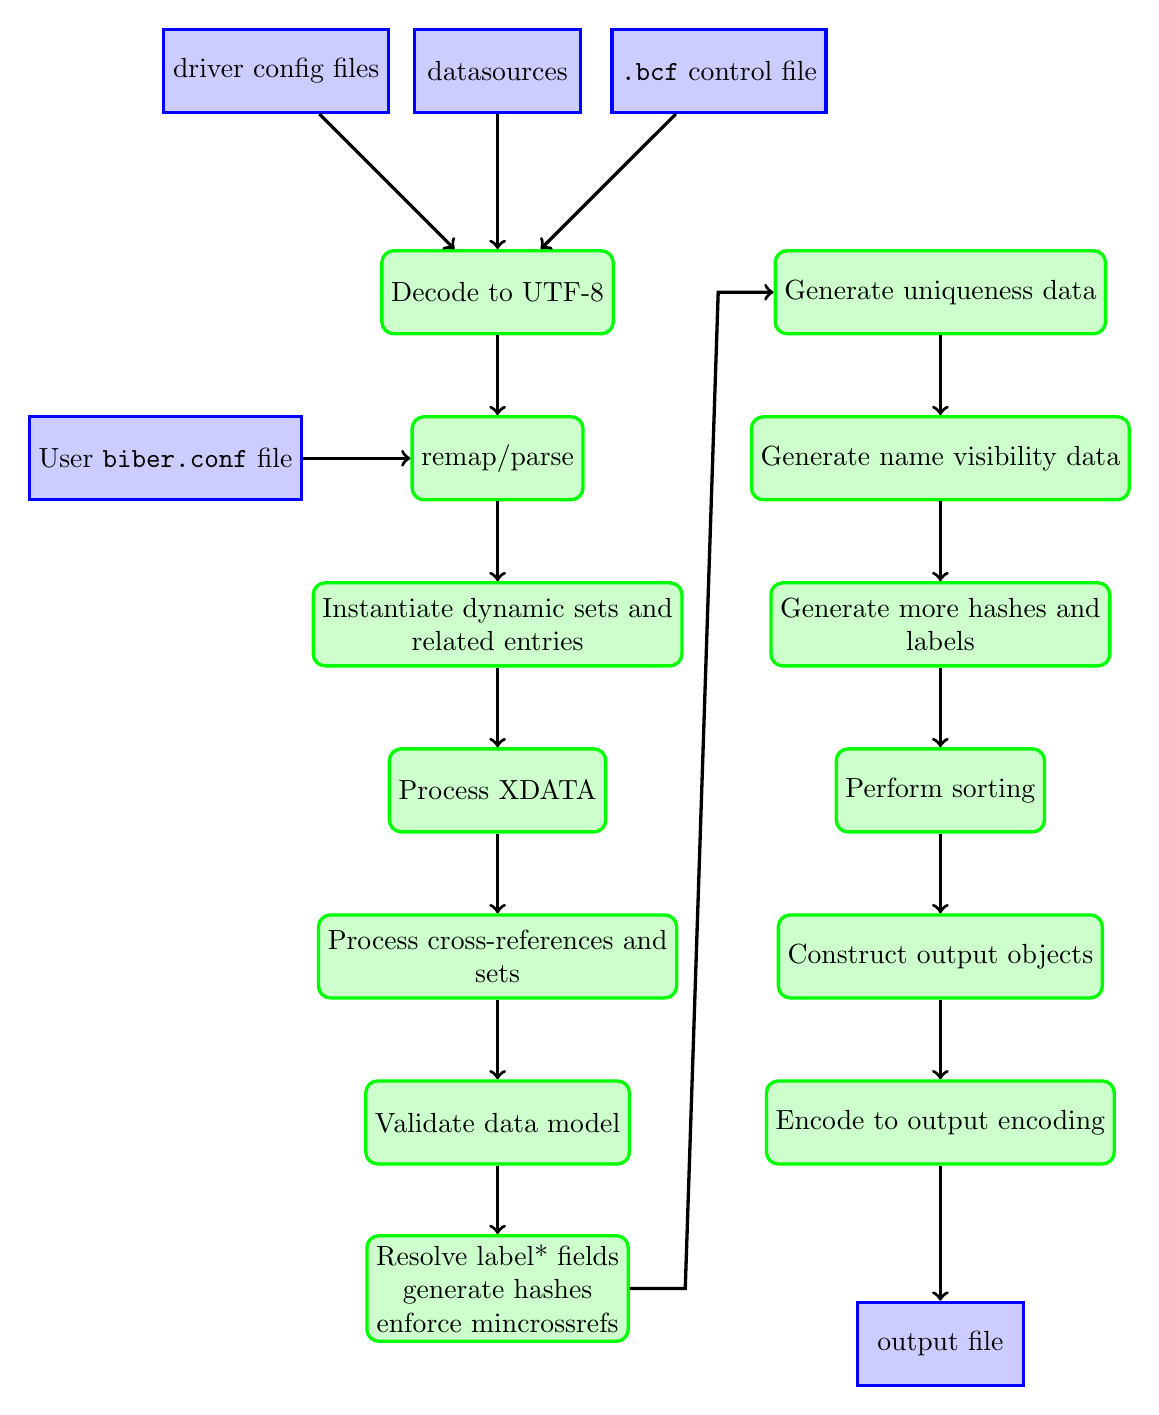
\begin{tikzpicture}
    \node[file] (dcfs) {driver config files};
    \node[file] (dsfiles) [right of=dcfs,node distance=8em]{datasources};
    \node[file] (bcf) [right of=dsfiles,node distance=8em] {\texttt{.bcf} control file};
    \node[funit] (decode) [below of=dsfiles,node distance=8em] {Decode to UTF-8} edge [<-,very thick] (dsfiles) edge [<-,very thick] (dcfs) edge [<-,very thick] (bcf);
    \node[funit] (mapp) [below of=decode,node distance=6em] {remap/parse} edge [<-,very thick] (decode);
    \node[file] (config) [left of=mapp,node distance=12em] {User \texttt{biber.conf} file} edge [->,very thick] (mapp);
    \node[funit] (dyn) [below of=mapp,node distance=6em] {Instantiate dynamic sets and\\related entries} edge [<-,very thick] (mapp);
    \node[funit] (xdata) [below of=dyn,node distance=6em] {Process XDATA} edge [<-,very thick] (dyn);
    \node[funit] (crossrefs) [below of=xdata,node distance=6em] {Process cross-references and\\sets} edge [<-,very thick] (xdata);
    \node[funit] (validate) [below of=crossrefs,node distance=6em] {Validate data model} edge [<-,very thick] (crossrefs);
    \node[funit] (pre) [below of=validate,node distance=6em] {Resolve label* fields\\generate hashes\\enforce mincrossrefs} edge [<-,very thick] (validate);
    \node[funit] (unique) [right of=decode,node distance=16em] {Generate uniqueness data};
    \draw[->,very thick] (pre.east) -- ($ (pre.east) + (2em,0) $) -- ($ (unique.west) - (2em,0) $) -- (unique.west);
    \node[funit] (visible) [below of=unique,node distance=6em] {Generate name visibility data} edge [<-,very thick] (unique);
    \node[funit] (post) [below of=visible,node distance=6em] {Generate more hashes and\\labels} edge [<-,very thick] (visible);
    \node[funit] (sort) [below of=post,node distance=6em] {Perform sorting} edge [<-,very thick] (post);
    \node[funit] (output) [below of=sort,node distance=6em] {Construct output objects} edge [<-,very thick] (sort);
    \node[funit] (encode) [below of=output,node distance=6em] {Encode to output encoding} edge [<-,very thick] (output);
    \node[file] (bbl) [below of=encode,node distance=8em] {output file} edge [<-,very thick] (encode);
  \end{tikzpicture}
  \caption{Overview of Biber's main functional units}
  \label{fig:overview}
\end{figure}

It may be useful to know something about the different routes a datasource
entry can take as it passes through Biber.

\begin{enumerate}
\item\label{list:cited} All cited entries which are subsequently found in a
  datasource are instantiated in the internal Biber data model.
\item Some uncited entries on which cited entries depend are
  instantiated in the internal Biber data model:
  \begin{itemize}
  \item Entries with entrytype \verb+XDATA+ which are referenced from cited
    entries.
    \item Entries mentioned in the \verb+CROSSREF+ or \verb+XREF +field of a cited entry
      (unless they are also cited themselves in which case they are already
      instantiated as per item \ref{list:cited} above).
      \item Clones of entries mentioned as a «related» entry of a cited
        entry\footnote{This is done to 
          implement the «related» entry feature which does not currently
          have a Bib\LaTeX\ interface.}.
      \item Members of sets, either explicit \verb+SET+ entrytype entries or
        dynamic sets.
  \end{itemize}
\item Some uncited but instantiated entries are promoted to cited
  status so that they make it into the output:
  \begin{itemize}
  \item Entries instantiated by being members of a set.
  \item Entries instantiated by being mentioned as an \verb+CROSSREF+ are
    promoted to cited status if \verb+CROSSREF+'ed or \verb+XREF+'ed at
    least \verb+mincrosref+ times.
  \item Clones of entries mentioned as a «related» entry of a cited entry.
  \end{itemize}
\item Some of these auto-cited entries have the «dataonly» option set on
  them so that Bib\LaTeX\ will only use them for data and will not output
  them to the bibliography:
  \begin{itemize}
  \item Clones of entries mentioned as a «related» entry of a cited entry.
  \end{itemize}
\end{enumerate}

\subsection{Performance}

Biber can't really be compared with Bib\TeX\ in any meaningful
way performance-wise. Biber is written in Perl and does a
\emph{great} deal more than Bib\TeX\ which is written in C. One of
Biber's test cases is a 2150 entry, 15,000 line \verb+.bib+ file
which references a 630 entry macros file with a resulting 160 or so page (A4)
formatted bibliography. This takes Biber under 3 minutes to process on
on a reasonable computer. This is perfectly acceptable, especially for a
batch program.

\subsection{Acknowledgements}

François Charette originally wrote Biber. Philip Kime joined in
the development in 2009.

\section{Use}

Firstly, please note that Biber will \emph{not} attempt to sanitise
the content of Bib\TeX\ data sources. That is, don't expect it to
auto-escape any \TeX\ special characters like «\verb+&+» or «\verb+%+» which
it finds in, for example, your \verb+TITLE+ fields. It used to do this in
earlier versions in some cases but as of version 0.9, it doesn't because
it's fraught with problems and leads to inconsistent expectations and
behaviour between different data source types. In your Bib\TeX\ data
sources, please make sure your entries are legal \TeX\ code.

Running \verb+biber --help+ will display all options and a brief
description of each. This is the most useful brief source of usage
information. Biber returns an exit code of 0 on success or 1 if
there was an error.

Most Biber options can be specified in long or short format. When
mentioning options below, they are referred to as
«\verb+long form|short form+» when an option has both a long and short
form. As usual with such options, when the option requires an argument, the
long form is followed by an equals sign «\verb+=+» and then the argument,
the short form is followed by a space and then the argument. For example,
the \verb+--configfile|-g+ option can be given in two ways:

\begin{verbatim}
biber --configfile=somefile.conf
biber -g somefile.conf
\end{verbatim}

With the \verb+backend=biber+ option, Bib\LaTeX\ switches its backend
interface and passes all options and information relevant to Biber's
operation in a control file with extension \verb+.bcf+\footnote{Bib\LaTeX\ Control
  File}. This is conceptually equivalent to the \verb+.aux+ file which
\LaTeX\ uses to pass information to Bib\TeX. The \verb+.bcf+ file is
XML and contains many options and settings which configure how Biber
is to process the bibliography and generate the \verb+.bbl+ file.

The usual way to call Biber is simply with the \verb+.bcf+ file
as the only argument. Bib\LaTeX\ always writes the control file with
a \verb+.bcf+ extension. Specifying the «\verb+.bcf+» extension to
Biber is optional. Assuming a control file called
\verb+test.bcf+, the following two commands are equivalent:

\begin{verbatim}
biber test.bcf
biber test
\end{verbatim}

\subsection{Options and config file}
Bib\LaTeX\ options which Biber needs to know about are passed
via the \verb+.bcf+ file. See Table \ref{tab:bltxopts} for the Bib\LaTeX\
options which Biber uses and also for the scopes which are supported
for each option. Biber also has its own options which are set using
the following resource chain, given in decreasing precedence order:\\[2ex]

\begin{table}
\begin{center}
\small
\begin{tabular}{lllll}
\toprule
Bib\LaTeX\ option & Global & Per-type & Per-entry\\
\midrule
alphaothers        & \checkmark & \checkmark &  \\
dataonly           &   & \checkmark  & \checkmark\\
inheritance        & \checkmark &   &  \\
labelalpha         & \checkmark & \checkmark &  \\
labelalphatemplate & \checkmark & \checkmark &  \\
labelnamespec      & \checkmark & \checkmark &  \\
labelnumber        & \checkmark & \checkmark &  \\
labelyear          & \checkmark & \checkmark &  \\
labelyearspec      & \checkmark & \checkmark &  \\
maxalphanames      & \checkmark & \checkmark & \checkmark\\
maxbibnames        & \checkmark & \checkmark & \checkmark\\
maxcitenames       & \checkmark & \checkmark & \checkmark\\
maxitems           & \checkmark & \checkmark & \checkmark\\
minalphanames      & \checkmark & \checkmark & \checkmark\\
minbibnames        & \checkmark & \checkmark & \checkmark\\
mincitenames       & \checkmark & \checkmark & \checkmark\\
minitems           & \checkmark & \checkmark & \checkmark\\
presort            & \checkmark & \checkmark & \checkmark\\
singletitle        & \checkmark & \checkmark &  \\
skipbib            &   & \checkmark & \checkmark\\
skiplab            &   & \checkmark & \checkmark\\
skiplos            &   & \checkmark & \checkmark\\
sortalphaothers    & \checkmark & \checkmark &  \\
sortexclusion      &   & \checkmark &  \\
sorting            & \checkmark &   &  \\
sortlos            & \checkmark &   &  \\
structure          & \checkmark &   &  \\
uniquelist         & \checkmark & \checkmark & \checkmark\\
uniquename         & \checkmark & \checkmark & \checkmark\\
useauthor          & \checkmark & \checkmark & \checkmark\\
useeditor          & \checkmark & \checkmark & \checkmark\\
useprefix          & \checkmark & \checkmark & \checkmark\\
usetranslator      & \checkmark & \checkmark & \checkmark\\
\bottomrule
\end{tabular}
\end{center}
\caption{Bib\LaTeX\ options which Biber uses}
\label{tab:bltxopts}
\end{table}

\noindent command line options $\rightarrow$\\
\hspace*{1em}\verb+biber.conf+ file $\rightarrow$\\
\hspace*{2em}\verb+.bcf+ file$\rightarrow$\\
\hspace*{3em}Biber hard-coded defaults\\[2ex]

\noindent Users do not need to care directly about the contents or format of the
\verb+.bcf+ file as this is generated from the options which they specify
via Bib\LaTeX. The config file is a place to set commonly used
command-line options and also to set options which cannot be set on the
command line.

The configuration file is by default called \verb+biber.conf+ but this can
be changed using the \verb+--configfile|-g+ option. Unless
\verb+--configfile|-g+ is used, the config file is
looked for in the following places, in decreasing order of preference:\\[2ex]

\noindent \verb+biber.conf+ in the current directory $\rightarrow$\\
\hspace*{1em}\verb+$HOME/.biber.conf+ $\rightarrow$\\
\hspace*{2em}\verb+$XDG_CONFIG_HOME/biber/biber.conf+ $\rightarrow$\\
\hspace*{3em}\verb+$HOME/Library/biber/biber.conf+ (Mac OSX only)\\
\hspace*{3em}\verb+$APPDATA/biber.conf+ (Windows only) $\rightarrow$\\
\hspace*{4em}the output of «\verb+kpsewhich biber.conf+» (if available on the
system)\\[2ex]

\noindent The config file is XML. Here Below is
an example config file which displays the Biber defaults:

\begin{lstlisting}[language=xml]
<?xml version="1.0" encoding="UTF-8"?>
<config>
  <bblencoding>UTF-8</bblencoding>
  <bibencoding>UTF-8</bibencoding>
  <bblsafechars>0</bblsafechars>
  <bblsafecharsset>base</bblsafecharsset>
  <bltxml>0</bltxml>
  <collate>1</collate>
  <collate_options>
    <option name="level" value="4"/>
  </collate_options>
  <debug>0</debug>
  <decodecharsset>base</decodecharsset>
  <fastsort>0</fastsort>
  <graph>0</graph>
  <mincrossrefs>0</mincrossrefs>
  <nodieonerror>0</nodieonerror>
  <nolog>0</nolog>
  <nostdmacros>0</nostdmacros>
  <nosort>
    <!-- strip prefices like 'al-' when sorting name fields -->
    <option name="type_names" value="\A\p{L}{2}\p{Pd}"/>
    <!-- strip diacritics when sorting name fields -->
    <option name="type_names" value="[\x{2bf}\x{2018}]"/>
  </nosort>
  <onlylog>0</onlylog>
  <quiet>0</quiet>
  <sortcase>true</sortcase>
  <sortlocale>en_US.utf8</sortlocale>
  <sortupper>true</sortupper>
  <trace>0</trace>
  <validate_config>0</validate_config>
  <validate_control>0</validate_control>
  <validate_structure>0</validate_structure>
  <wraplines>0</wraplines>
</config>
\end{lstlisting}

\noindent In practice, the most commonly used options will be set via
Bib\LaTeX\ macros in your document and automatically passed to Biber
via the \verb+.bcf+ file. Certain options apply only to Biber and can
only be set in the config file, particularly the more complex
options. Most options are simple tags. Exceptions are the
\verb+nosort+ and \verb+collate_options+ options which are slightly
more complex and can have sub-options as shown. A much more complex
option is the \verb+sourcemap+ option which is not set by default and
which is described in section \ref{map}.

\subsubsection{The \texttt{sourcemap} option}\label{map}

The supplied data source drivers implement a default mapping from data
source entrytypes and fields into the Bib\LaTeX\ data
model\footnote{The Bib\LaTeX\ data model is currently static and
  defined in the Bib\LaTeX\ manual. In the future (Bib\LaTeX\
  2.x), the data model will be dynamically defined by the user.}. If you
want to override or augment the driver mappings you can use the \verb+sourcemap+
option which makes it possible to, for example, have a data source with
non-standard entrytypes or fields and to have these automatically mapped
into other entrytypes/fields without modifying your data source.
Essentially, this alters the source data stream which
Biber uses to build the internal Bib\LaTeX\ data model. So, you
are not constrained such that you must map into the Bib\LaTeX\ data
model. Of course, if you don't, it's likely that your exotic new fields
will be ignored by Biber because they are not valid in the
Bib\LaTeX\ data model. In Bib\LaTeX\ 2.x, you will be able to
re-define the internal Bib\LaTeX\ data model and pass this to
Biber which will use it internally. Figure \ref{fig:biber-mdf} is a
graphical overview of the data flow for data model information. In
Bib\LaTeX\ 2.x, the greyed static Bib\LaTeX\ data model will be
replaced by a dynamic data model read from the \verb+.bcf+ control file.
See Figure \ref{fig:overview} for a more complete overview of
Biber's processing steps.

\begin{figure}[!htpb]
  \centering\small
  \begin{tikzpicture}
    \node[file] (dsfile) {datasource};
    \node[funit] (remap) [below of=dsfile, node distance=8em] {remap} edge [<-,dashed] (dsfile);
    \node[file] (dcf) [left of=remap, node distance=10em] {data model mapping\\from driver config file} edge [->,dashed] (remap);
    \node[file] (conf) [below of=remap,  node distance=7em] {data model mapping\\from Biber config file} edge [->,dashed] (remap);
    \node[funit] (parser) [right of=remap, node distance=8em] {parser} edge [<-,very thick] (remap);
    \node[funit] (validation) [right of=parser, node distance=8em] {validation} edge [<-,very thick] (parser);
    \node[file] (hard) [above of=validation, node distance=8em] {static Bib\LaTeX\\data model} edge [->,dashed] (parser) edge [->,dashed] (validation);
    \node[file] (bbl) [right of=parser, node distance=16em] {output file} edge [<-,very thick] (validation);
    \node[rectangle, draw=gray, fill=grey!40, opacity=0.4, fit=(hard), inner sep=1em] {};
  \end{tikzpicture}
  \caption{Model data flow in Biber}
  \label{fig:biber-mdf}
\end{figure}

The \verb+sourcemap+ option can only be set in the config file
and not on the command line as it has a complex structure. This
option allows you to perform various data source mapping
tasks which can be useful for pre-processing data which you do not
generate yourself:

\begin{itemize}
\item Map data source entrytypes to different entrytypes,
  optionally also adding new fields to the entry.
\item Map data source fields to different fields,
  optionally also adding new fields to the entry. This is basically a
  one$\rightarrow$many field mapping. You can also limit field
  mappings to specific data source entrytypes.
\item As a special case of the above, you can map data source fields
  to null, effectively removing them from the input stream.
\item Modify the contents of a field using standard Perl regular expression
  match and replace.
\item Restrict mappings to entries coming from particular data sources
  which you defined in \verb+\addresource{}+ macros.
\end{itemize}

\noindent The format of the \verb+sourcemap+ option section in the
config file is described below, followed by examples which will make
everything clear. Items in \textcolor{red}{red} are not
literal, they are descriptive meta-values which are explained in the
accompanying text. Items in \textcolor{blue}{blue} are optional within
their parent section. The general structure is:

\lstset{showspaces=false}
\begin{lstlisting}[language=xml,escapechar=+,mathescape=true]
<sourcemap>
  <maps datatype="+\textcolor{red}{driver$_1$}+" map_overwrite="1|0">
    <map$_1$ maptype="entrytype|field" +\textcolor{blue}{map\_overwrite="1|0"}+> ... </map$_1$>
               $\vdots$
    <map$_n$ maptype="entrytype|field" +\textcolor{blue}{map\_overwrite="1|0"}+> ... </map$_n$>
  </maps>
         $\vdots$
  <maps datatype="+\textcolor{red}{driver$_n$}+" map_overwrite="1|0">
    <map$_1$ maptype="entrytype|field" +\textcolor{blue}{map\_overwrite="1|0"}+> ... </map$_1$>
               $\vdots$
    <map$_n$ maptype="entrytype|field" +\textcolor{blue}{map\_overwrite="1|0"}+> ... </map$_n$>
  </maps>
</sourcemap>
\end{lstlisting}

\noindent Here, \textcolor{red}{\texttt{driver$_1$}}\ldots
\textcolor{red}{\texttt{driver$_n$}} are the names of valid Biber data
source drivers (see section \ref{dcf}). One thing to note here is the
\verb+map_overwrite+ attribute. This must be present and have a value of
\verb+0+ or \verb+1+. It determines whether, for this driver mapping
section, whether you may overwrite existing fields when adding new fields
or mapping them. This attribute can be overridden on a per-map basis, see
below. A warning will be issued either way saying whether an existing field
will or will not be overwritten. Only one mapping---the first mapping to
match a given entry---will be used (since the mappings modify the entries).

There are two types of mappings you can apply to your datasources:

\begin{itemize}
\item Entrytype mapping
\item Field mapping
\end{itemize}

\noindent An entrytype mapping allows you to do one or more of the
following:

\begin{itemize}
\item Map an entrytype to another entrytype
\item Add extra fields to all entries
\item Add extra fields to entries of a given entrytype
\item Restrict the changes to entries coming from particular datasources
\end{itemize}

\noindent A field mapping allows you to do one or more of the
following:

\begin{itemize}
\item Map a field to another field
\item Change the contents of a field
\item Add extra fields to entries with particular fields
\item Restrict the changes to entries coming from particular
  datasources
\item Restrict the changes to entries of a particular entrytype
\end{itemize}

\noindent These facilities are explained in more detail below, with examples.

\minisec{Entrytype mapping}

\lstset{showspaces=false,showstringspaces=false}
\begin{lstlisting}[language=xml,escapechar=+,mathescape=true]
<map maptype="entrytype" +\textcolor{blue}{map\_overwrite="0|1"}+>
  +\textcolor{blue}{<per\_datasource>\textcolor{red}{datasource}</per\_datasource>}+
  <map_pair map_source="+\textcolor{red}{source-entrytype}+"
              +\textcolor{blue}{map\_target="\textcolor{red}{target-entrytype}"}+/>
  +\textcolor{blue}{<also\_set map\_field="\textcolor{red}{set-field}"}+
              +\textcolor{blue}{map\_value="\textcolor{red}{set-value}"}+
              +\textcolor{blue}{map\_null="1"}+
              +\textcolor{blue}{map\_origentrytype="1"/>}+
</map>
\end{lstlisting}

\noindent An \verb+entrytype+ element performs a mapping of one or more
mapping «pairs» of entrytypes. Each pair consists of a \verb+map_pair+
element with a \verb+map_source+ attribute with value
\textcolor{red}{\texttt{source-entrytype}} and an optional
\verb+map_target+ attribute with value
\textcolor{red}{\texttt{target-entrytype}}. The target is
optional as you might want to simply modify entries of a certain entrytype
without changing the entrytype. The
\textcolor{red}{\texttt{source-entrytype}} is mandatory and can be the
string «\verb+*+» which means «all entrytypes». Mappings for specific
entrytypes override the generic «\verb+*+» type. The
rules for an entrytype mapping are:\\[1ex]

\begin{itemize}
\item Change the \textcolor{red}{\texttt{source-entrytype}} to
  \textcolor{red}{\texttt{target-entrytype}}, if defined.
\item If there are any \textcolor{red}{\texttt{datasource}}s named in
  \textcolor{blue}{\texttt{per\_datasource}} elements, this mapping only applies to entries
  coming from the named \textcolor{red}{\texttt{datasource}}s. There can be
  multiple \textcolor{blue}{\texttt{per\_datasource}} elements each specifying one of the
  datasource names given in a Bib\LaTeX\ \verb+\addbibresource+ macro.
\item There can be one or more \textcolor{blue}{\texttt{also\_set}} elements which each specify
  a behaviour for an entry field. The \textcolor{blue}{\texttt{map\_field}} attribute is
  mandatory and specified the field \textcolor{red}{\texttt{set-field}} in
  the entry to map. One and only one of these other attributes are then
  mandatory:
  \begin{itemize}
    \item \textcolor{blue}{\texttt{map\_value}} --- The
      \textcolor{red}{\texttt{set-field}} is set to
      \textcolor{red}{\texttt{set-value}}
    \item \textcolor{blue}{\texttt{map\_null}} --- The field is mapped to
      null, that is, it is deleted from the input stream completely. This
      is useful for ignoring field in datasources which are badly formatted
      or which you don't even want Bib\LaTeX\ to see at all.
      \item \textcolor{blue}{\texttt{map\_origentrytype}} --- The
        \textcolor{red}{\texttt{set-field}} is set to the value of the
        \linebreak\textcolor{red}{\texttt{source-entrytype}} name.
  \end{itemize}
\end{itemize}

\noindent Here are some examples:

\begin{lstlisting}[language=xml,escapechar=+,mathescape=true]
<map maptype="entrytype">
  <per_datasource>example1.bib</per_datasource>
  <per_datasource>example2.bib</per_datasource>
  <map_pair map_source="*"/>
  <also_set map_field="KEYWORDS" map_value="keyw1, keyw2"/>
</map>
\end{lstlisting}

\noindent This would add a \verb+KEYWORDS+ field with value «\verb+keyw1, keyw2+»
to entries of any entrytype which are found in either the
\verb+examples1.bib+ or \verb+examples2.bib+ files. This assumes that the
Bib\LaTeX\ source contains \verb+\addresource{example1.bib}+ and
\verb+\addresource{example2.bib}+.

\begin{lstlisting}[language=xml,escapechar=+,mathescape=true]
<map maptype="entrytype" map_overwrite="0">
  <map_pair map_source="CHAT" map_target="CUSTOMA"/>
  <also_set map_field="TYPE" map_origentrytype="1"/>
</map>
\end{lstlisting}

\noindent Any \verb+CHAT+ entrytypes would become \verb+CUSTOMA+ entrytypes and 
would automatically have a \verb+TYPE+ field set to 
«chat» unless the \verb+TYPE+ field already existed in the entry.

\begin{lstlisting}[language=xml,escapechar=+,mathescape=true]
<map maptype="entrytype">
  <map_pair map_source="ARTICLE"/>
  <map_pair map_source="BOOK"/>
  <also_set map_field="ABSTRACT" map_null="1"/>
  <also_set map_field="NOTE" map_value="Auto-created this field"/>
</map>
\end{lstlisting}

\noindent Any \verb+ARTICLE+ or \verb+BOOK+ entrytypes would have their \verb+ABSTRACT+
fields removed and a \verb+NOTE+ field added with value «Auto-created this field».
\bigskip
\minisec{Field mapping}

\begin{lstlisting}[language=xml,escapechar=+,mathescape=true]
<map maptype="field" +\textcolor{blue}{map\_overwrite="0|1"}+>
  +\textcolor{blue}{<per\_datasource>\textcolor{red}{datasource}</per\_datasource>}+
  +\textcolor{blue}{<per\_type>\textcolor{red}{entrytype}</per\_type>}+
  <map_pair map_source="+\textcolor{red}{source-field}+"
              +\textcolor{blue}{map\_target="\textcolor{red}{target-field}"}+/>
              +\textcolor{blue}{map\_match="\textcolor{red}{match-regexp}"}+
              +\textcolor{blue}{map\_replace="\textcolor{red}{replace-regexp}"}+
              +\textcolor{blue}{map\_null="1"}+/>
  +\textcolor{blue}{<also\_set map\_field="\textcolor{red}{set-field}"}+
              +\textcolor{blue}{map\_value="\textcolor{red}{set-value}"}+
              +\textcolor{blue}{map\_null="1"}+
              +\textcolor{blue}{map\_origfield="1"}+
              +\textcolor{blue}{map\_origfieldval="1"/>}+
</map>
\end{lstlisting}

\noindent A \verb+field+ element performs a mapping of one or more
mapping «pairs» of fields. Each pair consists of a \verb+map_pair+ element with a
\verb+map_source+ attribute with value \textcolor{red}{\texttt{source-field}} and an optional
\verb+map_target+ attribute with
value \textcolor{red}{\texttt{target-field}}. The target is optional as
you might want to simply modify certain fields without mapping to other fields.
The \textcolor{red}{\texttt{source-field}} is
mandatory. If there are more than one \verb+map_pair+ rules for the
same \textcolor{red}{\texttt{source-field}}, the last one to be
defined takes precedence (but note the special case of map/replace
pairs below). The rules for a field mapping are:\\[1ex]

\begin{itemize}
\item Change the \textcolor{red}{\texttt{source-field}} to
  \textcolor{red}{\texttt{target-field}}, if defined.
\item Remove the \textcolor{red}{\texttt{source-field}} if
  \textcolor{blue}{\texttt{map\_null}} is set.
\item If \textcolor{blue}{\texttt{map\_match}} is defined but
  \textcolor{blue}{\texttt{map\_replace}} is not, only apply the
  mapping if the \textcolor{red}{\texttt{source-field}} matches
  \textcolor{blue}{\texttt{map\_match}}.
\item Perform a Perl Regular Expression match and replace on the value of
  \textcolor{red}{\texttt{source-field}} if
  \textcolor{blue}{\texttt{map\_match}} and
  \textcolor{blue}{\texttt{map\_replace}} are defined. You may use (and almost certainly
  will want to use) parentheses for back-references in \textcolor{blue}{\texttt{map\_replace}}.
  Do not quote the regular expressions in any way---it's not
  necessary. There may be multiple \verb+map_pair+ elements for the
  same \textcolor{red}{\texttt{source-field}} within a \verb+map+
  element. Any \textcolor{blue}{\texttt{map\_match}} and
  \textcolor{blue}{\texttt{map\_replace}} pairs for the same
  \textcolor{red}{\texttt{source-field}} are cumulative and will all
  be applied to the field, in order.
\item If there are any \textcolor{red}{\texttt{datasource}}s named in
  \textcolor{blue}{\texttt{per\_datasource}} elements, this mapping only applies to entries
  coming from the named \textcolor{red}{\texttt{datasource}}s. There can be
  multiple \textcolor{blue}{\texttt{per\_datasource}} elements each specifying one of the
  datasource names given in a Bib\LaTeX\ \verb+\addbibresource+ macro.
\item If there are any \textcolor{red}{\texttt{entrytypes}}s named in
  \textcolor{blue}{\texttt{per\_type}} elements, this mapping only applies to entries
  of the named \textcolor{red}{\texttt{entrytypes}}s.
\item There can be one or more \textcolor{blue}{\texttt{also\_set}} elements which each specify
  a behaviour for an entry field. The \textcolor{blue}{\texttt{map\_field}} attribute is
  mandatory and specified the field \textcolor{red}{\texttt{set-field}} in
  the entry to map. One and only one of these other attributes are then
  mandatory:
  \begin{itemize}
    \item \textcolor{blue}{\texttt{map\_value}} --- The
      \textcolor{red}{\texttt{set-field}} is set to
      \textcolor{red}{\texttt{set-value}}
    \item \textcolor{blue}{\texttt{map\_null}} --- The field is mapped to
      null, that is, it is deleted from the input stream completely. This
      is useful for ignoring field in datasources which are badly formatted
      or which you don't even want Bib\LaTeX\ to see at all.
      \item \textcolor{blue}{\texttt{map\_origfield}} --- The
        \textcolor{red}{\texttt{set-field}} is set to the value of the
        \textcolor{red}{\texttt{source-field}} name.
      \item \textcolor{blue}{\texttt{map\_origfieldval}} --- The
        \textcolor{red}{\texttt{set-field}} is set to the original value
        (before, for example, any regular expression match/replace) of the
        \textcolor{red}{\texttt{source-field}}.
  \end{itemize}
\end{itemize}

\noindent Here are some examples:

\begin{lstlisting}[language=xml,escapechar=:,mathescape=true]
<map maptype="field">
  <map_pair map_source="ABSTRACT" map_null="1"/>
  <map_pair map_source="CONDUCTOR" map_target="NAMEA"/>
  <map_pair map_source="GPS" map_target="USERA"/>
</map>
\end{lstlisting}

\noindent This removes any \verb+ABSTRACT+ fields from any entry, changes
\verb+CONDUCTOR+ fields to \verb+NAMEA+ fields and changed \verb+GPS+
fields to \verb+USERA+ fields

\begin{lstlisting}[language=xml,escapechar=:,mathescape=true]
<map maptype="field">
  <per_datasource>examples.bib</per_datasource>
  <per_type>MISC</per_type>
  <per_type>UNPUBLISHED</per_type>
  <map_pair map_source="ADDENDUM" map_null="1"/>
  <map_pair map_source="NOTE" map_null="1"/>
</map>
\end{lstlisting}

\noindent Here we remove any \verb+ADDENDUM+ or \verb+NOTE+ fields in
\verb+MISC+ or \verb+UNPUBLISHED+ entries coming from the
\verb+examples.bib+ datasource.

\begin{lstlisting}[language=xml,escapechar=:,mathescape=true]
<map maptype="field">
  <map_pair map_source="PUBMEDID" map_target="EPRINT"/>
  <also_set map_field="EPRINTTYPE" map_origfield="1"/>
  <also_set map_field="USERD" map_value="Some string of things"/>
</map>
\end{lstlisting}

\noindent This maps \verb+PUBMEDID+ fields to \verb+EPRINT+ fields, sets
the \verb+EPRINTTYPE+ field to «pubmedid» and also sets the \verb+USERD+
field to the string «Some string of things».

\begin{lstlisting}[language=xml,escapechar=:,mathescape=true]
<map maptype="field">
  <per_datasource>examples.bib</per_datasource>
  <map_pair map_source="SERIES"
            map_match=":\textbackslash A\textbackslash d$\ast$(.+):"
            map_replace=":\textbackslash L\$1:"/>
</map>
\end{lstlisting}

\noindent Here, the contents of the \verb+SERIES+
field have leading numbers stripped and the remainder of the contents
lowercased.

\begin{lstlisting}[language=xml,escapechar=:,mathescape=true]
<map maptype="field">
  <map_pair map_source="TITLE"
            map_match=":Collected\textbackslash s+Works.+Freud:"/>
  <also_set map_field="KEYWORDS" map_value="freud"/>
</map>
\end{lstlisting}

\noindent Here, if the \verb+TITLE+ field matches a particular
regexp, we set a special keyword so we can, for example, make a
references section just for certain items.

\begin{lstlisting}[language=xml,escapechar=:,mathescape=true]
<map maptype="field">
  <map_pair map_source="AUTHOR"
            map_match="Smith, Bill" map_replace="Smith, William"/>
  <map_pair map_source="AUTHOR"
            map_match="Jones, Baz" map_replace="Jones, Barry"/>
</map>
\end{lstlisting}

\noindent Here, we use multiple match/replace for the same field to
regularise some inconstant name variants. Bear in mind that the
results of a match/replace feed into the match of the next
match/replace as they are processed in serial. This is not usually an
issue if the matches are mutually exclusive.
\bigskip
\minisec{Other datasource types}
For data sources other than Bib\TeX, (e.g. \verb+ris+,
\verb+endnotexml+ and \verb+zoterordfxml+), the source entrytypes and
fields are usually very differently modelled and named. For example, here
is how to drop \verb+subject+ fields from various entrytypes in Zotero XML
RDF format data sources:

\begin{lstlisting}[language=xml,escapechar=+,mathescape=true]
<maps datatype="zoterordfxml" map_overwrite="1">
  <map maptype="field">
    <per_type>journalArticle</per_type>
    <per_type>book</per_type>
    <per_type>bookSection</per_type>
    <map_pair map_source="dc:subject" map_null="1"/>
  </map>
</maps>
\end{lstlisting}

\noindent Or here, mapping journal articles into \verb+REPORT+ entries for
Endnote XML format data sources within a particular data source.

\begin{lstlisting}[language=xml,escapechar=+,mathescape=true]
<maps datatype="endnotexml" map_overwrite="1">
  <map>
    <per_datasource>endnote.xml</per_datasource>
    <map_pair map_source="journal Article" map_target="REPORT"/>
  </map>
</maps>
\end{lstlisting}

\noindent Or here, dropping the \verb+N2+ field from \verb+RIS+
datasources, which are commonly used for abstracts:

\begin{lstlisting}[language=xml,escapechar=+,mathescape=true]
<maps datatype="ris" map_overwrite="1">
      <map maptype="field">
        <map_pair map_source="N2" map_null="1"/>
      </map>
</maps>
\end{lstlisting}
\bigskip
\subsubsection{The \texttt{nosort} option}\label{nosort}

The value of the \verb+nosort+ option can only be set in the config file
and not on the command line. This is because the values are Perl regular
expressions and would need special quoting to set on the command line. This
can get a bit tricky on some OSes (like Windows) so it's safer to set them
in the config file. In any case, it's unlikely you would want to set them
for particular Biber runs; they would more likely be set as your
personal default and thus they would naturally be set in the config file
anyway. \verb+nosort+ allows you to ignore parts of a field for sorting.
This is done using Perl regular expressions which specify what to
ignore in a field. You can specify as many patterns as you like for a
specific field. Also available are some field type aliases so you can, for
example, specify patterns for all name fields or all title fields. These
field types all begin with the string «\verb+type_+», see Table
\ref{tab:nst}.

\begin{table}
\begin{center}
\small
\begin{tabular}{ll}
\toprule
Alias & Fields\\
\midrule
type\_name & author\\
          & afterword\\
          & annotator\\
          & bookauthor\\
          & commentator\\
          & editor\\
          & editora\\
          & editorb\\
          & editorc\\
          & foreword\\
          & holder\\
          & introduction\\
          & namea\\
          & nameb\\
          & namec\\
          & shortauthor\\
          & shorteditor\\
          & translator\\
type\_title & booktitle\\
           & eventtitle\\
           & issuetitle\\
           & journaltitle\\
           & maintitle\\
           & origtitle\\
           & title\\
\bottomrule
\end{tabular}
\end{center}
\caption{\texttt{nosort} option field type aliases}
\label{tab:nst}
\end{table}

For example, this option can be used to ignore diacritic marks and prefices
in names which should not be considered when sorting. Given (the default):

\begin{lstlisting}[language=xml]
<nosort>
  <!-- strip prefices like 'al-' when sorting names -->
  <option name="type_names" value="\A\p{L}{2}\p{Pd}"/>
  <!-- strip diacritics when sorting names -->
  <option name="type_names" value="[\x{2bf}\x{2018}]"/>
</nosort>
\end{lstlisting}

\noindent and the Bib\TeX\ data source entry:

\begin{verbatim}
AUTHOR = {{al-Hasan}, ʿAlī},
\end{verbatim}

\noindent the prefix «al-» and the diacritic «ʿ» will not be considered
when sorting. See the Perl regular expression manual page for
details of the regular expression syntax\footnote{\url{http://perldoc.perl.org/perlre.html}}.

You may specify any number of \verb+option+ elements. If a
\verb+nosort+ option is found for a specific field, it will override
any option for a type which also covers that field.

Here is another example. Suppose you wanted to ignore «The» at the
beginning of a \verb+TITLE+ field when sorting, you could add this to your
\verb+biber.conf+:

\begin{lstlisting}[language=xml]
<nosort>
  <option name="title" value="\AThe\s+"/>
</nosort>
\end{lstlisting}

\noindent If you wanted to do this for all title fields listed in Table
\ref{tab:nst}, then you would do this:

\begin{lstlisting}[language=xml]
<nosort>
  <option name="type_title" value="\AThe\s+"/>
</nosort>
\end{lstlisting}

\noindent \textbf{Note:} \verb+nosort+ can be specified for most fields but
not for things like dates and special fields as that wouldn't make much sense.
\bigskip
\subsubsection{The \texttt{collate\_options} option}

The \verb+collate_options+ option has format similar to
\verb+nosort+. See Section \ref{coll} for details about the option,
here is an example of a config file setting:

\begin{lstlisting}[language=xml]
<collate_options>
  <option name="level" value="3"/>
  <option name="table" value="/home/user/data/otherkeys.txt"/>
</collate_options>
\end{lstlisting}
\bigskip
\subsection{Input/Output File Locations}

\subsubsection{Control file}\label{loc:cf}

The control file is normally passed as the only argument to biber. It is
searched for in the following locations, in decreasing order of
priority:\\[2ex]

\noindent Absolute filename $\rightarrow$\\
\hspace*{1em}In the \verb+--output_directory+, if specified$\rightarrow$\\
\hspace*{2em}Relative to current directory$\rightarrow$\\
\hspace*{3em}Using \verb+kpsewhich+, if available

\subsubsection{Data sources}

Local data sources of type «file» are searched for in the following
locations, in decreasing order of priority:\\[2ex]

\noindent Absolute filename $\rightarrow$\\
\hspace*{1em}In the \verb+--output_directory+, if specified$\rightarrow$\\
\hspace*{2em}Relative to current directory$\rightarrow$\\
\hspace*{3em}In the same directory as the control file$\rightarrow$\\
\hspace*{4em}Using \verb+kpsewhich+ for supported formats, if available\\[2ex]

\noindent Remote file data sources (beginning with \verb+http://+ or
\verb+ftp://+) are retrieved to a temp file and processed as normal. Users
do not specify explicitly the bibliography database files; they are passed
in the \verb+.bcf+ control file, which is constructed from the
Bib\LaTeX\ «\verb+\addbibresource{}+» macros.

\subsection{Logfile}

By default, the logfile for biber will be named \verb+\jobname.blg+,
so, if you run

\begin{verbatim}
  biber <options> test.bcf
\end{verbatim}

\noindent then the logfile will be called «\verb+test.blg+». Like the
\verb+.bbl+ output file, it will be created in the
\verb+--output_directory|-c+, if this option is defined. You can
override the logfile name by using the \verb+--logfile+ option:

\begin{verbatim}
  biber --logfile=lfname test.bcf
\end{verbatim}

\noindent results in a logfile called «\verb+lfname.blg+».\\

\noindent \textbf{Warning}: be careful if you are expecting Biber to
write to directories which you don't have appropriate permissions to. This
is more commonly an issue on non-Windows OSes. For example, if you rely on
\verb+kpsewhich+ to find your database files which are in system \TeX\
directories, you may well not have write permission there so Biber
will not be able to write the \verb+.bbl+. Use the \verb+--outfile|-O+
option to specify the location to write the \verb+.bbl+ to in such cases.

\subsection{Collation and Localisation}\label{coll}

Biber takes care of collating the bibliography for
Bib\LaTeX. It writes entries to the \verb+.bbl+ file sorted by a
completely customisable set of rules which are passed in the
\verb+.bcf+ file by Bib\LaTeX. Biber has two ways of performing
collation:\\[2ex]

\biberex{--collate|-C}
  \noindent The default. This option makes Biber use the Perl
  \verb+Unicode::Collate+ module for collation which implements the full UCA (Unicode
  Collation Algorithm). It also has CLDR (Common Locale Data
  Repository) tailoring to deal with cases which are not covered by the
  UCA. It is a little slower than \verb+--fastsort|-f+ but the
  advantages are such that it's rarely worth using \verb+--fastsort|-f+\\[1ex]

\biberex{--fastsort|-f}
  \noindent Biber will sort using
  the OS locale collation tables. The drawback for this method is that special
  collation tailoring for various languages are not implemented in the
  collation tables for many OSes. For example, few OSes correctly sort 'å'
  before 'ä' in the Swedish (\verb+sv_SE+) locale. If you are using a
  common latin alphabet, then this is probably not a problem for you.\\[2ex]

\noindent The locale used for collation is determined by the following resource
chain which is given in decreasing precedence order:\\[2ex]

\noindent\verb+--collate_options|-c+ (e.g. \verb+-c 'locale => "de_DE"'+) $\rightarrow$\\
\hspace*{1em}\verb+--sortlocale|-l+ $\rightarrow$\\
\hspace*{2em}\verb+LC_COLLATE+ environment variable $\rightarrow$\\
\hspace*{3em}\verb+LANG+ environment variable $\rightarrow$\\
\hspace*{4em}\verb+LC_ALL+ environment variable\\[2ex]

\noindent With the default \verb+--collate|-C+ option, the locale will
be used to look for a collation tailoring for that locale. It will generate an
informational warning if it finds none. This is not a problem as the vast
majority of collation cases are covered by the standard UCA and many
locales neither have nor need any special collation tailoring.

With the \verb+--fastsort|-f+ option, the locale will be
used to locate an OS locale definition to use for the collation. This
may or may not be correctly tailored, depending on the locale and the OS.

Collation is by default case sensitive. You can turn this
off globally using the Biber option \verb+--sortcase=false+ or from
Bib\LaTeX\ using its option\linebreak[4]\verb+sortcase=false+. The option can also
be defined per-field so you can sort some fields case sensitively and
others case insensitively. See the Bib\LaTeX\ manual.

\verb+--collate|-C+ by default collates uppercase before lower.
You can reverse this globally for all sorting using the Biber option
\verb+--sortupper=false+ or from\linebreak[4]Bib\LaTeX\ by using its option
\verb+sortupper=false+. The option can also be defined per-field so you can
sort some fields uppercase before lower and others lower before upper. See the
Bib\LaTeX\ manual. Be aware though that some locales rightly enforce a
particular setting for this (for example, Danish). You will be able to
override it but Biber will warn you if you do. \verb+sortupper+ has
no effect when using \verb+--fastsort|-f+--you are at the mercy of what
your OS locale does.

There are in fact many options to \verb+Unicode::Collate+
which can tailor the collation in various ways in
addition to the locale tailoring which is automatically performed.
Users should see the the documentation to the module for the various
options, most of which the vast majority of users will never
need\footnote{For details on the various options, see
  \url{http://search.cpan.org/search?query=Unicode\%3A\%3ACollate&mode=all}}.
Options are passed using the \verb+--collate_options|-c+ option as a
single quoted string, each option separated by comma, each key and
value separated by «\verb+=>+». See examples.

\subsubsection{Examples}

\biberex{biber}

\noindent Call biber using all settings from the \verb+.bcf+ generated from the
\LaTeX\ run. Case sensitive UCA sorting is performed taking the locale
for tailoring from the environment if no \verb+sortlocale+ is defined in
the \verb+.bcf+

\biberex{biber --sortlocale=de_DE}

\noindent Override any locale setting in the \verb+.bcf+ or
the environment.

\biberex{biber --fastsort}

\noindent Use slightly quicker internal sorting routine. This uses the OS locale
files which may or may not be accurate.

\biberex{biber --sortcase=false}

\noindent Case insensitive sorting.

\biberex{biber --sortupper=false --collate_options="backwards => 2"}

\noindent Collate lowercase before upper and collate French accents in
reverse order at UCA level 2.

\subsection{Encoding of files}

Biber takes care of reencoding the data source data as
necessary. In normal use, Bib\LaTeX\ passes its
\verb+bibencoding+ option value to Biber via the \verb+.bcf+
file. It also passes the value of its \verb+texencoding+ option (which
maps to Biber's \verb+--bblencoding|-E+ option) the default value
of which depends on which \TeX\ engine and encoding packages you are
using (see Bib\LaTeX\ manual for details).

\noindent Biber performs the following tasks:

\begin{enumerate}
\item Decodes the data source into UTF-8 if it is not UTF-8 already
\item Decodes \LaTeX\ character macros into UTF-8 if \verb+--bblencoding|-E+
  is UTF-8
\item Encodes the output so that the \verb+.bbl+ is in
  the encoding that \verb+--bblencoding|-E+ specifies
\item Warns if it is asked to output to the \verb+.bbl+ any UTF-8
  decoded \LaTeX\ character macros which are not in the
  \verb+--bblencoding|-E+ encoding. Replaces with a suitable \LaTeX\ macro
\end{enumerate}

\noindent Normally, you do not need to set the encoding options on the
Biber command line as they are passed in the \verb+.bcf+ via the
information in your Bib\LaTeX\ environment. However, you can override
the \verb+.bcf+ settings with the command line. The resource chain for
encoding settings is, in decreasing order
of preference:\\[2ex]

\noindent\verb+--bibencoding|-e+ and \verb+--bblencoding|-E+ $\rightarrow$\\
\hspace*{1em}Biber config file $\rightarrow$\\
\hspace*{2em}\verb+.bcf+ control file

\subsubsection{\LaTeX\ macro decoding}\label{ldecode}

\noindent As mentioned above, Biber sometimes converts \LaTeX\
character macros into UTF-8. In fact there are two situations in which
this occurs.

\begin{enumerate}
\item When \verb+--bblencoding|-E+ is UTF-8
\item Always for internal sorting purposes
\end{enumerate}

\noindent This decoding is very useful but take note of the following
two scenarios, which relate to each of the two situations in which
\LaTeX\ macro decoding occurs:
\bigskip
\minisec{Decoding when output is UTF-8}
If you are using PDF\LaTeX\ and \verb+\usepackage[utf8]{inputenc}+, it
is possible that the UTF-8 characters resulting from Biber's
internal \LaTeX\ character macro decoding break \verb+inputenc+. This is
because \verb+inputenc+ does not implement all of UTF-8, only a
commonly used subset.

An example--if you had \verb+\DJ+ in your \verb+.bib+ data source,
Biber decodes this correctly to «Đ» and this breaks \verb+inputenc+
because it doesn't understand that UTF-8 character. The real solution here
is to switch to a \TeX\ engine with full UTF-8 support like \XeTeX\ or Lua\TeX\
as these don't use or need \verb+inputenc+. However, you can also try the
\verb+--bblsafechars+ option which will try to convert any UTF-8 chars into
\LaTeX\ macros on output. For information on the \verb+--bblsafechars+
option, see section \ref{lencode}.
\bigskip
\minisec{Decoding for internal sorting}

If your \verb+bblencoding+ is not UTF-8, and you are using some UTF-8
equivalent \LaTeX\ character macros in your \verb+.bib+ data source, then some
\verb+.bbl+ fields (currently only \verb+\sortinit{}+) might end up
with invalid characters in them, according to the \verb+.bbl+
encoding. This is because some fields must be generated from the final
sorting data which is only available after the \LaTeX\ character macro
decoding step.

For example, suppose you are using PDF\LaTeX\ with\\
\verb+\usepackage[latin1]{inputenc}+ and the following Bib\TeX\
data source entry:

\begin{verbatim}
@BOOK{citekey1,
  AUTHOR = {{\v S}imple, Simon},
}
\end{verbatim}

\noindent With normal \LaTeX\ character macro decoding, the
\verb+{\v S}+ is decoded into «Š» and so with name-first sorting,
\verb+\sortinit{}+ would be «Š». This is an invalid character in
latin1 encoding and so the \verb+.bbl+ would be broken. In such cases
when \verb+\sortinit{}+ is a char not valid in the \verb+bblencoding+,
Biber tries to replace the character with a suitable \LaTeX\
macro. The solution is really to use UTF-8 \verb+.bbl+ encoding whenever
possible. In extreme cases where even with UTF-8 encoding,
the char is not recognised by \LaTeX\ due to an incomplete UTF-8
implementation (as with \verb+inputenc+), this might also mean
switching \TeX\ engines to one that supports full UTF-8.

\subsubsection{\LaTeX\ macro encoding}\label{lencode}

The opposite of decoding; converting UTF-8 characters into \LaTeX\ macros.
You can force this with the \verb+--bblsafechars+ option which will do a
generally good job of making your \verb+.bbl+ plain ASCII. It can be useful
in certain edge cases where your bibliography introduces characters which
can't be handled by your main document. See section \ref{ldecode} above for
an example such case.

A common use case for \LaTeX\ macro encoding is when the bibliography
data source is not ASCII but the \verb+.tex+ file is and so this case
is automated for you: if the Bib\LaTeX\ option «\verb+texencoding+»
(which corresponds to the Biber option «\verb+--bblencoding|-E+») is
set to an ASCII encoding («\verb+ascii+» or «\verb+x-ascii+») and
«\verb+--bibencoding|-e+» is not ASCII, Biber will automatically set
\verb+--bblsafechars+.

See also the \verb+biber --help+ output for the \verb+--bblsafecharsset+
and \linebreak[4]\verb+--decodecharsset+ options which can customise the set
of conversion rules to use. The characters and macros which Biber
maps during encoding and decoding are documented\footnote{\url{https://sourceforge.net/projects/biblatex-biber/files/biblatex-biber/\biberversion/documentation/utf8-macro-map.html}}.
\bigskip
\subsubsection{Examples}

\biberex{biber}

\noindent Set \verb+bibencoding+ and \verb+bblencoding+ from the
config file or \verb+.bcf+

\biberex{biber --bblencoding=latin2}

\noindent Encode the \verb+.bbl+ as latin2, overriding the
\verb+.bcf+

\biberex{biber --bblsafechars}

\noindent Set \verb+bibencoding+ and \verb+bblencoding+ from the
config file or \verb+.bcf+. Force encoding of UTF-8 chars to \LaTeX\
macros using default conversion set

\biberex{biber --bblencoding=ascii}

\noindent Encode the \verb+.bbl+ as ascii, overriding the
\verb+.bcf+. Automatically sets \verb+--bblsafechars+ to force UTF-8
to \LaTeX\ macro conversion

\biberex{biber --bblencoding=ascii --bblsafecharsset=full}

\noindent Encode the \verb+.bbl+ as ascii, overriding the
\verb+.bcf+. Automatically sets \verb+--bblsafechars+ to force UTF-8
to \LaTeX\ macro conversion using the full set of conversions

\biberex{biber --decodecharsset=full}

\noindent Set \verb+bibencoding+ and \verb+bblencoding+ from the
config file or \verb+.bcf+. Use the full \LaTeX\ macro to UTF-8
conversion set because you have some more obscure character macros in
your \verb+.bib+ data source which you want to sort correctly

\biberex{biber -u}

\noindent Shortcut alias for \verb+biber --bibencoding=UTF-8+

\biberex{biber -U}

\noindent Shortcut alias for \verb+biber --bblencoding=UTF-8+

\subsection{Editor Integration}

Here is some information on how to integrate Biber into some of the
more common editors

\subsubsection{Emacs}

Emacs has the powerful AUC\TeX\ mode for editing \TeX\ and running
compilations. Updated files for AUC\TeX\ 11.86 are available here:\\[2ex]

\noindent\url{http://sourceforge.net/projects/biblatex-biber/files/auctex-biber.zip}\\[2ex]

\noindent Drop the \verb+.el+ files in the \verb+.zip+ file over the
ones in your AUC\TeX\ installation tree, delete the corresponding
\verb+.elc+ files and run \verb+M-0 M-x byte-recompile-directory+ and
give the path of your AUC\TeX\ main install directory where the new
files reside. Hopefully these modifications will make it into the
official AUC\TeX\ distributions soon.

The additions augment AUC\TeX\ in the following ways:

\begin{itemize}
\item Adds font-lock support for most Bib\LaTeX\ macros
\item Auto-detects whether you are using Biber with Bib\LaTeX\
\item Can detect whether dependencies like data sources have changed without
  them being open in Emacs
\item Understands Bib\LaTeX\ and Biber messages so that
  AUC\TeX\ will prompt you with the best default command to run next
  when using \verb+C-cC-c+
\end{itemize}

\subsubsection{\TeX works}

It's very easy to add Biber support to \TeX works. In the Preferences,
select the Typesetting tab and then add a new Processing Tool as in Figure
\ref{fig:biber-texworks}.

\begin{figure}[!htpb]
  \centering
  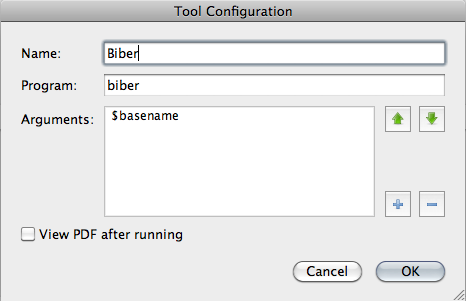
\includegraphics[width=4in,keepaspectratio=true]{biber-texworks.png}
  \caption{Screenshot of \TeX works processing tool setup for Biber}
  \label{fig:biber-texworks}
\end{figure}

\subsection{Bib\TeX\ macros and the \texttt{MONTH} field}

Bib\TeX\ defines macros for month abbreviations
like «\verb+jan+», «\verb+feb+» etc. Biber also does this,
defining them as numbers since that is what Bib\LaTeX\ wants. In
case you are also defining these yourself (although if you are only
using Bib\LaTeX, there isn't much point), you will get macro
redefinition warnings from the \verb+btparse+ library. You can turn
off Biber's macro definitions to avoid this by using the option
\verb+--nostdmacros+.

Biber will look at any \verb+MONTH+ field in a Bib\TeX\ data
source and if it's not a number as Bib\LaTeX\ expects (because it
wasn't one of the macros as mentioned above or these macros were disabled
by \verb+--nostdmacros+), it will try to turn it into the right number in
the \verb+.bbl+. If you only use Bib\LaTeX\ with your Bib\TeX\
data source files, you should probably make any \verb+MONTH+ fields be the
numbers which Bib\LaTeX\ expects.

\subsection{Biber data source drivers}\label{dcf}

Biber uses a modular data source driver model to provide access
to supported data sources. The drivers are responsible for mapping
driver entry types and fields to the Bib\LaTeX\ model. This is
aided by a driver configuration file (\verb+.dcf+). The information in
this file for each driver can be found in the driver documentation folder on
SourceForge\footnote{\url{https://sourceforge.net/projects/biblatex-biber/files/biblatex-biber/\biberversion/documentation/drivers}}. This
file shows you which handlers the driver uses for different fields and
what certain entry types and fields are aliased to in the
Bib\LaTeX\ data model. This is not fantastically useful to know
without knowing also what the named driver handlers do specifically but there
is a «description» section which mentions any special handling and
general comments on the driver. You should read the documentation for
the drivers you use to get an idea of how Biber handles your
data. Data model mapping is an imprecise art
and the drivers are where the necessarily messy parts of Biber
live. Most data source models are not designed with typesetting in
mind and are usually not fine-grained enough to provide the sorts of
information that Bib\LaTeX\ needs. Biber does its best to
obtain as much meaningful information from a data source as possible.
Currently supported data sources drivers are:

\begin{itemize}
\item Bib\TeX\ --- Bib\TeX\ data files
\item \verb+endnotexml+ --- Endnote XML export format, version $\geq$ Endnote X1
\item \verb+ris+ --- Research Information Systems format
\item \verb+zoterordfxml+ --- Zotero RDF XML format, version 2.0.9
\end{itemize}

\subsection{Visualising the Output}

The option \verb+--graph+ will cause Biber to write a
GraphViz\footnote{\url{http://www.graphviz.org}} \verb+.dot+ file instead
of a \verb+.bbl+. This file graphs the bibliographic data as it exists
after all processing. You can transform this file using the \verb+dot+
program from GraphViz to generate a high quality graphical representation
of the data in a format of your choice. A good output format choice with
\verb+dot+ is SVG\footnote{Scalable Vector Graphics} which can be viewed in
any modern web browser. This format has the advantage of tooltips and Biber
uses these to give you more information on connections between entries:
hover the cursor on an arrow in the output and it will tell you what it
means. To output in SVG, use this command after installing GraphViz:

\begin{verbatim}
dot -Tsvg <file>.dot -o <file>.svg
\end{verbatim}

\noindent The \verb+--graph+ option takes a comma delimited string as
argument. The elements of this string define the information to include in
the \verb+.dot+ output graph. The valid sub-options are shown in Table
\ref{tab:graphopts}. If the \verb+--graph+ option is given with no argument
then the default is

\begin{verbatim}
--graph=crossref,section,xdata,xref
\end{verbatim}

\begin{table}
\begin{center}
\small
\begin{tabular}{ll}
\toprule
Sub-option & Description\\
\midrule
crossref & Show crossreference relationships\\
field    & Show fields within entries\\
related  & Show related entries and clones\\
section  & Show sections\\
xdata    & Show XDATA relationships\\
xref     & Show XREF relationships\\
\bottomrule
\end{tabular}
\end{center}
\caption{Valid sub-options for the \texttt{graph} option}
\label{tab:graphopts}
\end{table}

\noindent As with all options which take an optional value, be careful to
terminate the options if you use \verb+--graph+ with the implied defaults,
otherwise Biber will interpret the \verb+.bcf+ file name as the value of
the option:

\begin{verbatim}
biber --graph -- file[.bcf]
\end{verbatim}

\noindent Without the option terminating \verb+--+, Biber would try to use
the \verb+.bcf+ filename as the value of the \verb+--graph+ option. Figure
\ref{fig:graphkey} is a key to the elements included to the \verb+.dot+
output.

\begin{figure}[!htpb]
  \centering\small
  \begin{tikzpicture}
    \node[rectangle, black, draw=black, fill=centry, align=center] (centry)
    {<key> (<entrytype>)\\\\Cited entry};
    \node[rectangle, black, draw=black, fill=ncentry, align=center]
    (ncentry) [right of=centry, node distance=11em] {<key>
      (<entrytype>)\\\\Uncited entry};
    \node[rectangle, black, draw=black, fill=doentry, align=center]
    (doentry) [right of=ncentry, node distance=11em] {<key>
      (<entrytype>)\\\\dataonly entry};
    \node[rectangle, black, draw=black, fill=section, align=center]
    (section) [below of=centry, node distance=5em] {Section
      <number>\\\\Section};
    \node[rectangle, black, draw=black, fill=set, align=center]
    (set) [right of=section, node distance=11em] {<key> (SET)\\\\Entry set};

    % CROSSREF
    \node[black] (cr1) [below of=section, node distance=6em] {A};
    \node[black] (cr2) [right of=cr1, node distance=20em] {B};
    \path (cr1) edge [->, color=crossref, very thick] node[auto, black] {B inherits by CROSSREF from A} (cr2);

    % XREF
    \node[black] (xr1) [below of=cr1, node distance=5em] {A};
    \node[black] (xr2) [right of=xr1, node distance=20em] {B};
    \path (xr1) edge [->, color=xref, style=dashed, very thick] node[auto, black] {B inherits by XREF from A} (xr2);

    % XDATA
    \node[black] (xd1) [below of=xr1, node distance=5em] {A};
    \node[black] (xd2) [right of=xd1, node distance=20em] {B};
    \path (xd1) edge [->, color=xdata, very thick] node[auto, black] {B inherits by XDATA from A} (xd2);

    % RELATED
    \node[black] (re1) [below of=xd1, node distance=5em] {A};
    \node[black] (re2) [right of=re1, node distance=20em] {B};
    \path (re1) edge [->, color=related, very thick] node[auto, black]
    {A is a related entry of B} (re2);

    % CLONE
    \node[black] (c1) [below of=re1, node distance=5em] {A};
    \node[black] (c2) [right of=c1, node distance=20em] {B};
    \path (c1) edge [->, color=clone, style=dashed, very thick] node[auto, black]
    {B is a clone of A} (c2);
  \end{tikzpicture}
  \caption{Key to \texttt{.dot} output format}
  \label{fig:graphkey}
\end{figure}

\section{Binaries}\label{binaries}

Biber is a Perl application which relies heavily on quite a few
modules. It is packaged as a stand-alone binary using the excellent
\verb+PAR::Packer+ module which can pack an entire Perl tree plus
dependencies into one file which acts as a stand-alone binary and is
indistinguishable from such to the end user. You can also simply download
the Perl source and run it as a normal Perl program which
requires you to have a working Perl 5.14+ installation and the
ability to install the pre-requisite modules. You would typically only do
this if you wanted to keep up with all the bleeding-edge git commits before
they had been packaged as a binary. Almost all users will not want to do
this and should use the binaries from their \TeX\ distribution or downloaded
directly from SourceForge in case they need to use a more recent binary
than is included in their \TeX\ distribution.

The binary distributions of biber are made using the Perl \verb+PAR::Packer+
module. They can be used as a normal binary but have some behaviour which
is worth noting:

\begin{itemize}
\item Don't be worried by the size of the binaries. \verb+PAR::Packer+ essentially
  constructs a self-extracting archive which unpacks the needed files first.
\item On the first run of a new version (that is, with a specific hash),
  they actually unpack themselves to a temporary location which varies by
  operating system. This unpacking can take a little while and only happens
  on the first run of a new version. \textbf{Please don't kill the process
    if it seems to take some time to do anything on the first run of a new
    binary}. If you do, it will not unpack everything and it will almost
  certainly break Biber. You will then have to delete your binary
  cache (see section \ref{bc} below) and re-run the Biber executable
  again for the first time to allow it to unpack properly.
\end{itemize}

\subsection{Binary Caches}\label{bc}

\verb+PAR::Packer+ works by unpacking the required files to a cache
location. It only does this on the first run of a binary 
by computing a hash of the binary and comparing it with
the cache directory name which contains the hash. So, if you run
several versions of a binary, you will end up with several cached
trees which are never used. This is particularly true if you are regularly
testing new versions of the Biber binary. It is a good idea to
delete the caches for older binaries as they are not needed and can take up
a fair bit of space. The caches are located in a temporary location which
varies from OS to OS. The cache name is:\\[1ex]

\noindent\verb+par-<username>/cache-<hash>+ (Linux/Unix/OSX)\\
\verb+par-<username>\cache-<hash>+ (Windows)\\[1ex]

\noindent The temp location is not always obvious but these are sensible
places to look (where \verb+*+ can vary depending on username):

\begin{itemize}
\item \verb+/var/folders/*/*/*/+ (OSX, local GUI login shell)
\item \verb+/var/tmp/+ (OSX (remote ssh login shell), Unix)
\item \verb+/tmp/+ (Linux)
\item \verb+C:\Documents and Settings\<username>\Local Settings\Temp+ (Windows/Cygwin)
\item \verb+C:\Windows\Temp+ (Windows)
\end{itemize}

\noindent To clean up, you can just remove the whole \verb+par-<username>+
directory/folder and then run the current binary again.

\subsection{Binary Architectures}

Binaries are available for many architectures, directly on SourceForge and
also via \TeX Live:

\begin{itemize}
\item \verb+linux_x86_32+
\item \verb+linux_x86_64+
\item \verb+MSWin32+
\item \verb+cygwin32+
\item \verb+darwin_x86_64+
\item \verb+darwin_x86_i386+
\item \verb+freebsd_x86+\tpb
\item \verb+freebsd_amd64+\tpb
\item \verb+solaris_x86+\tpb
\end{itemize}

\noindent If you want to run development versions, they are usually only
regularly updated for the core architectures which are not flagged as
third-party built above. If you want to regularly run the latest
development version, you should probably git clone the relevant branch and
run Biber as a pure perl program directly.

\subsection{Installing}

These instructions only apply to manually downloaded binaries. If
Biber came with your \TeX\ distribution just use it as normal.

Download the binary appropriate to you
OS/arch\footnote{\url{https://sourceforge.net/projects/biblatex-biber}}. Below
I assume it's on your desktop.

You have to move the binary to somewhere in you command-line or \TeX\ utility
path so that it can be found. If you know how to do this, just ignore the
rest of this section which contains some instructions for users who are
not sure about this.

\subsubsection{OSX}

If you are using the \TeX Live Mac\TeX\ distribution:

\begin{verbatim}
sudo mv ~/Desktop/biber /usr/texbin/
sudo chmod +x /usr/texbin/biber
\end{verbatim}

\noindent If you are using the macports \TeX Live distribution:

\begin{verbatim}
sudo mv ~/Desktop/biber /opt/local/bin/
sudo chmod +x /opt/local/bin/biber
\end{verbatim}

\noindent The «\verb+sudo+» commands will prompt you for your password.

\subsubsection{Windows}

The easiest way is to just move the executable into your \verb+C:\Windows+ directory since
that is always in your path. A more elegant is to put it somewhere in
your \TeX\ distribution that is already in your path. For example if you
are using MiK\TeX:

\begin{verbatim}
C:\Program Files\MiKTeX 2.9\miktex\bin\
\end{verbatim}

\subsubsection{Unix/Linux}

\begin{verbatim}
sudo mv ~/Desktop/biber /usr/local/bin/biber
sudo chmod +x /usr/local/bin/biber
\end{verbatim}

\noindent Make sure \verb+/usr/local/bin+ is in your PATH. Search Google for «set PATH
linux» if unsure about this. There are many pages about this, for example:
\url{http://www.cyberciti.biz/faq/unix-linux-adding-path/}


\subsection{Building}

Instructions for those who want/need to build an executable from the
Perl version. For this, you will need to have Perl 5.14+ with
the following modules:

\begin{itemize}
\item All Biber pre-requisites
\item \verb+PAR::Packer+ and all dependencies
\end{itemize}

\noindent You should have the latest CPAN versions of all required modules
as Biber is very specific in some cases about module versions and
depends on recent fixes in many cases. You can see if you have the
Biber Perl dependencies by the usual

\begin{verbatim}
perl ./Build.PL
\end{verbatim}

\noindent invocation in the Biber Perl distribution tree
directory. Normally, the build procedure for the binaries is as
follows\footnote{On UNIXequse systems, you may need to specify a full
  path to the scripts e.g. \texttt{./Build}}:

\begin{itemize}
\item Get the biber source tree from SF and put it on the architecture
  you are building for
\item cd to the root of the source tree
\item \verb+perl Build.PL+ (this will check your module
  dependencies)
\item \verb+Build test+
\item \verb+Build install+ (may need to run this as sudo on
  UNIXesque systems)
\item \verb+cd dist/<arch>+
\item \verb+build.sh+ (\verb+build.bat+ on Windows)
\end{itemize}

\noindent This leaves a binary called «\verb+biber-<arch>+» (also with
a «\verb+.exe+» extension on Windows/Cygwin) in your current directory.
The tricky part is constructing the information for the build
script. There are two things that need to be configured, both of
which are required by the \verb+PAR::Packer+ module:

\begin{enumerate}
\item A list of modules/libraries to include in the binary which are not
  automatically detected by the \verb+PAR::Packer+ dependency
  scanner
\item A list of extra files to include in the binary which are not
  automatically detected by the \verb+PAR::Packer+ dependency
  scanner
\end{enumerate}

\noindent To build Biber for a new architecture you need to
define these two things as part of constructing new build scripts:

\begin{itemize}
\item Make a new subfolder in the \verb+dist+ directory named after the
  architecture you are building for. This name is arbitrary but should
  be fairly obvious like «\verb+solaris-sparc-64+», for example.
\item Copy the \verb+biber.files+ file from an existing build
  architecture into this directory.
\item For all of the files with absolute pathnames in there (that is,
  ones we are not pulling from the Biber tree itself), locate these
  files in your Perl installation tree and put the correct path in the
  file.
\item Copy the build script from a vaguely similar architecture
  (i.e. Windows/non-Windows \ldots) to your new architecture
  directory. 
\item Change the \verb+--link+ options to point to where the required
  libraries reside on your system.
\item Change the \verb+--output+ option to name the resulting binary
  for your architecture.
\item Run the build script
\end{itemize}

\noindent The \verb+--link+ options can be a little tricky
sometimes. It is usually best to build without them once and then run
\verb+ldd+ (or OS equivalent) on the binary to see which
version/location of a library you should link to. You can also try
just running the binary and it should complain about missing libraries
and where it expected to find them. Put this path into the
\verb+--link+ option. The \verb+--module+ options are the same for all
architectures and do not need to be modified.
On architectures which have or can have case-insensitive file systems,
you should use the build script from either Windows or OSX as a reference
as these include a step to copy the main Biber script to a new name
before packing the binary. This is required as otherwise a spurious
error is reported to the user on first run of the binary due to a name
collision when it unpacks itself.

See the \verb+PAR+ wiki
page\footnote{\url{http://par.perl.org/wiki/Main_Page}} for FAQs and help
on building with \verb+PAR::Packer+. Take special note of the FAQs on
including libraries with the packed
binary\footnote{\url{http://par.perl.org/wiki/FAQ}, section entitled «My
  PAR executable needs some dynamic libraries»}.

\subsubsection{Testing a binary build}
You can test a binary that you have created by copying it to a machine
which preferably doesn't have \verb+perl+ at all on it. Running the binary with no
arguments will unpack it in the background and display the help. To really
test it without having \LaTeX\ available, get the two quick test files from
SourceForge\footnote{\url{https://sourceforge.net/projects/biblatex-biber/files/biblatex-biber/testfiles}},
put them in a directory and run Biber in that directory like this:

\begin{verbatim}
biber --validate_control --convert_control test
\end{verbatim}

\noindent This will run Biber normally on the test files plus it
will also perform an XSLT transform on the \verb+.bcf+ and
leave an HTML representation of it in the same directory thus testing the
links to the XML and XSLT libraries as well as the Bib\TeX\ parsing
libraries. The output should look something like this (may be differences
of Biber version and locale of course but there should be no errors
or warnings).

\begin{verbatim}
INFO - This is Biber 0.9.8
INFO - Logfile is 'test.blg'
INFO - BibLaTeX control file 'test.bcf' validates
INFO - Converted BibLaTeX control file 'test.bcf' to 'test.bcf.html'
INFO - Reading 'test.bcf'
INFO - Found 1 citekeys in bib section 0
INFO - Processing bib section 0
INFO - Looking for BibTeX format file 'test.bib' for section 0
INFO - Found BibTeX data file 'test.bib'
INFO - Decoding LaTeX character macros into UTF-8
INFO - Sorting list 'MAIN' keys
INFO - No sort tailoring available for locale 'en_GB.UTF-8'
INFO - Sorting list 'SHORTHANDS' keys
INFO - No sort tailoring available for locale 'en_GB.UTF-8'
INFO - Writing 'test.bbl' with encoding 'UTF-8'
INFO - Output to test.bbl
\end{verbatim}

\noindent There should now be these new files in the directory:

\begin{verbatim}
test.bcf.html
test.blg
test.bbl
\end{verbatim}


\end{document}
